%!TEX root = ../thesis.tex
%*******************************************************************************
%****************************** Optim2D Chapter **********************
%*******************************************************************************
\chapter{L-BFGS Optimisation of Phase-Only Hologram}\label{L-BFGS Optimisation of Phase-Only Hologram}

\graphicspath{{Chapter_Optim2D/Figs/}}

\textit{Note: The work in this chapter has been published in Ref. \cite{Sha2023}}\\\\

This chapter implements the limited-memory Broyden-Fletcher-Goldfarb-Shanno (L-BFGS) optimization method introduced in \cref{sec:L-BFGS} to generate phase-only computer-generated hologram (CGH) for both 2D and 3D targets. For 3D targets, instead of computing the full 3D reconstruction of the hologram at every iteration, a novel method called sequential slicing (SS) is proposed for partial evaluation of the hologram during optimization.

\section{Introduction}
% Holography, taking its name from the Greek word $o \lambda o \sigma $ (holos), meaning \textit{whole}, was first introduced in 1948 by Dennis Gabor \cite{Gabor1948}, originally named as \textit{wavefront reconstruction} \cite{Hecht2017}. It is a technology that can record and reconstruct the wavefront of three-dimensional (3D) objects. Similar to two-dimensional (2D) photography, the earliest holography uses a piece of film to record the diffraction pattern of an object, which can then reconstruct the wavefront showing that object. In order to generate hologram for objects that do not physically exist, computer-generated holography (CGH) emerged, where a hologram can be calculated through various algorithmic approaches and then displayed on a spatial light modulator (SLM) modulating a coherent light source, in order to reconstruct target images \cite{Cable2006,Seldowitz1987,Yang2009,Gerchberg1972}, either 2D or 3D, which can provide full depth cues at arbitrary angles instead of stereoscopic displays which need to re-compute the left-eye and right-eye images every time the position changes. So the multi-depth reconstruction ability is a major advantage of the holography technology.

Currently available spatial light modulators can only modulate either phase or amplitude, so algorithms are needed to compute amplitude-only or phase-only holograms, among which the phase-only holograms are usually preferred due to its higher energy efficiency. The classic algorithms include direct binary search \cite{Seldowitz1987}, simulated annealing \cite{Kirkpatrick1983} and Gerchberg-Saxton \cite{Gerchberg1972}, which is still widely used despite it being nearly 50 years old. With the developments in modern numerical optimization methods and computation power, advances in CGH algorithms can be made. Literature review has found some recent work that compute CGH using numerical optimization methods \cite{Zhang2017, Liu2020, Choi2021, Chen2021, Kadis2022}, but speed and quality are still the major challenges in multi-depth hologram generation. The most common multi-depth CGH optimization methods either evaluate their loss against the entire multi-depth 3D target, which is time-consuming, or evaluate the hologram for each plane and then sum the holograms, which introduces quality degradation.

This paper therefore extends on the previous research, which proved the ability of L-BFGS algorithm to generate phase-only hologram for a 2D image \cite{Sha2022}, and proposes the sequential slicing (SS) technique for the optimization of CGH for multi-depth 3D target, which evaluates the loss for a single slice at each iteration, aiming for quicker hologram generation with proper overall quality and low quality imbalance across the multiple depths enabled by the second-order nature of the L-BFGS optimization algorithm. The following sections start from the background knowledge of numerical optimization including L-BFGS algorithm, then introduces and carries out the optimization of multi-depth CGH with sequential slicing (SS) technique, with results analysed.



\section{Method}



The optimization algorithms used for CGH in this paper are GD and L-BFGS. The phase-only constraint of CGH can be easily applied by fixing a constant amplitude of the hologram, while keeping its phase varying and being the argument of optimization ($\textbf{x}$).

\begin{figure}[H]
	\centering
	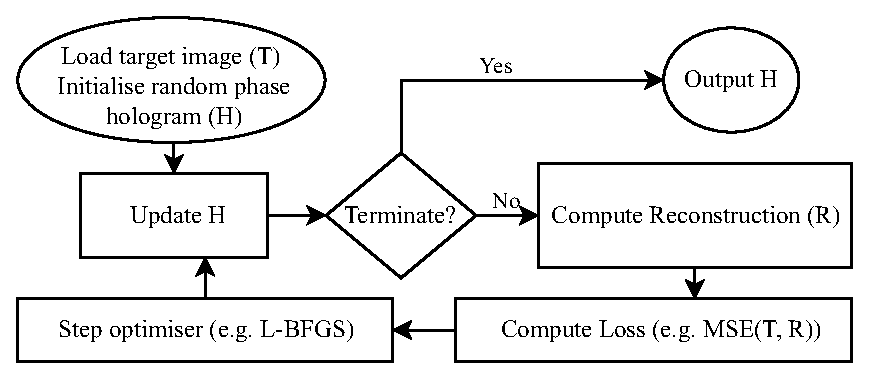
\includegraphics[width=\textwidth]{optim_flowchart_2D.eps}
	\caption{Flowchart of the optimisation process}
	\label{fig:optim_flowchart_2D}
\end{figure}




